\documentclass{article} % For LaTeX2e

\usepackage[preprint]{neurips_2024}

% Optional math commands from https://github.com/goodfeli/dlbook_notation.
\usepackage{hyperref}
\usepackage{url}
% \usepackage[numbers]{natbib}
\usepackage[utf8]{inputenc} % allow utf-8 input
\usepackage[T1]{fontenc}    % use 8-bit T1 fonts
% \usepackage[numbers]{natbib}
\usepackage{hyperref}       % hyperlinks           % simple URL typesetting
\usepackage{booktabs}       % professional-quality tables
\usepackage{algorithm}
\usepackage{algorithmic}
\usepackage{tikz}
\usetikzlibrary{arrows.meta,trees}

\usepackage{array}  
\usepackage{color}
\usepackage{newfloat}
\usepackage{listings}
\usepackage{booktabs}
\usepackage{float}
\usepackage{subfig}
\usepackage{tabularray}
\usepackage[most]{tcolorbox}
\usepackage{caption}
\usepackage{courier}
\usepackage{listings}
\usepackage{enumitem}
\usepackage{graphicx}
\usepackage{newfloat}
\usepackage{listings}
\usepackage{amssymb}   
\usepackage{amsmath}
\usepackage{tabularray}
%\usepackage{geometry}
\usepackage{xcolor}
\usepackage{makecell}
\usepackage{wrapfig}
\usepackage{multirow}

\title{DAMR: Efficient and Adaptive Context-Aware Knowledge Graph Question Answering with LLM-Guided MCTS}
\allowdisplaybreaks[4]
\newcommand{\method}{DAMR}



\author{%
  Yingxu Wang\\
  MBZUAI \\
  yingxv.wang@gmail.com
  \And
  Shiqi Fan\\
  PolyU\\
  fsq@mail.nwpu.edu.cn
  \And
  Mengzhu Wang\\
  Hebei University of Technology\\
  dreamkily@gmail.com
  \And
  Siyang Gao, Chao Wang\\
  CityU\\
  {siyangao@cityu.edu.hk, chanceycn@gmail.com}
  \And
  Nan Yin \\
  HKUST \\
  yinnan8911@gmail.com
}

\begin{document}


\maketitle
\begin{abstract}
Knowledge Graph Question Answering (KGQA) aims to interpret natural language queries and perform structured reasoning over knowledge graphs by leveraging their relational and semantic structures to retrieve accurate answers. 
Existing methods primarily follow either the retrieve-then-reason paradigm, which relies on Graph Neural Networks (GNNs) or heuristic rules to extract static candidate paths, or dynamic path generation strategies that employ large language models (LLMs) with prompting to jointly perform retrieval and reasoning. 
However, the former lacks adaptability due to static path extraction and the absence of contextual refinement, while the latter suffers from high computational costs and limited evaluation accuracy because of their dependence on fixed scoring functions and repeated LLM calls.
To address these issues, this paper proposes \textbf{D}ynamically \textbf{A}daptive \textbf{M}CTS-based \textbf{R}easoning (\method{}), a novel framework that integrates LLM-guided Monte Carlo Tree Search (MCTS) with adaptive path evaluation to enable efficient and context-aware KGQA. 
\method{} leverages MCTS as a backbone, where an LLM-based planner selects the top-$k$ semantically relevant relations at each expansion step to effectively reduce the search space. To enhance evaluation accuracy, we introduce a lightweight Transformer-based scorer that performs context-aware plausibility estimation by jointly encoding the question and relation sequence through cross-attention, thereby capturing fine-grained semantic shifts during multi-hop reasoning. Furthermore, to mitigate the scarcity of high-quality supervision, \method{} incorporates a dynamic pseudo-path refinement mechanism that periodically generates training signals from partial paths explored during search, enabling the scorer to continually adapt to the evolving distribution of reasoning trajectories.
Extensive experiments on multiple KGQA benchmarks show that \method{} significantly outperforms state-of-the-art methods. 
\end{abstract}


\section{Introduction}

Large Language Models (LLMs) have demonstrated impressive reasoning capabilities across diverse tasks, including mathematical problem solving~\citep{pei2025mathfusion,didolkar2024metacognitive}, commonsense inference~\citep{toroghi2024verifiable}, and open-domain question answering~\citep{zhao2023divknowqa}. 
Despite their generalization ability, LLMs often struggle in domain-specific scenarios due to the lack of grounded external knowledge, resulting in factual hallucinations and high inference costs~\citep{huang2025survey,wang2024factuality}. To address these limitations, recent efforts have explored integrating domain knowledge into LLM reasoning. A promising direction to overcome these limitations is Knowledge Graph Question Answering (KGQA)~\citep{dammu2025dynamic,saxena2020improving,choi2023nutrea}, which integrates relational structures into the reasoning process to provide factual grounding and structural interpretability. By combining the expressiveness of natural language with the precision of knowledge graphs, KGQA offers a scalable solution to improve factual consistency, reasoning transparency, and answer reliability~\citep{liu2025dual,yao2025learning}. 

Existing KGQA approaches can be broadly categorized into two paradigms according to how reasoning paths are constructed: retrieve-then-reason methods and dynamic path generation strategies. In the former, candidate paths are extracted prior to answer prediction, typically using Graph Neural Networks (GNNs) \citep{ma2025debate,yao2025learning} or rule-based heuristics \citep{fang2024karpa}. However, such methods exhibit limited adaptability, as GNNs fail to incorporate question-specific semantics during inference, while heuristic rules remain inherently inflexible and cannot support dynamic refinement of reasoning~\citep{liu2025dual,yao2025learning}. In contrast, dynamic path generation strategies unify retrieval and reasoning by constructing paths dynamically during question processing. These methods either leverage LLMs to iteratively generate paths through in-context learning or Chain-of-Thought (CoT)~\citep{sui2024fidelis,li2024framework}, or employ guided search techniques such as MCTS, where paths are incrementally expanded with a path scorer~\citep{ma2025deliberation,shen2025reasoning}. While offering greater flexibility, such approaches suffer from substantial computational overhead due to repeated LLM calls and limited evaluation accuracy, as static scorers cannot capture the evolving semantics of reasoning paths~\citep{chang2024survey,lee2024zero}.

This paper investigates the design of an adaptive KGQA framework to address challenges of computational inefficiency and limited path evaluation accuracy in dynamic reasoning. However, developing such a framework raises three key challenges: (1) \textit{How to modularize reasoning to reduce LLM overuse in search?} Inefficiency in dynamic KGQA stems from repeatedly invoking LLMs for relation retrieval and reasoning in multi-hop path construction~\citep{shen2025reasoning,long2025enhancing}. Although methods such as CoT and MCTS enable flexible exploration, they bind LLMs to every decision step, causing high inference cost and poor scalability. The challenge is to design a modular framework that leverages LLMs efficiently, guiding search without direct involvement at each step. (2) \textit{How to accurately evaluate evolving reasoning paths?} As multi-hop paths are incrementally constructed, their semantics evolve with each added relation and context. Yet existing methods rely on static scoring or shallow similarity metrics that fail to capture these semantic shifts~\citep{xu2024llm,sui2024fidelis}. This highlights the challenge of designing a path evaluation model that adaptively captures fine-grained changes conditioned on both the question and evolving relation sequence. (3) \textit{How to train a reliable evaluation model with limited supervision?} Accurate path ranking requires a well-calibrated scorer, yet dynamic reasoning generates many incomplete paths with only a few valid ones. This results in imbalanced, noisy supervision, especially for multi-hop questions where successful trajectories are scarce. While reinforcement learning has been explored~\citep{ma2024coevolving,zhai2024fine}, it suffers from sparse rewards and unstable optimization. The key challenge is to construct reliable learning signals from limited supervision to support adaptive scorer training.

% This paper investigates the design of an adaptive KGQA framework to address the challenges of computational inefficiency and limited path evaluation accuracy in dynamic reasoning. However, developing such a framework presents several key challenges: (1) \textit{How to modularize reasoning to reduce LLM overuse during search?} A major source of computational inefficiency in dynamic KGQA lies in repeatedly invoking LLMs for both relation retrieval and reasoning during multi-hop path construction~\citep{shen2025reasoning,long2025enhancing}. While methods such as CoT and MCTS provide flexible exploration, they tightly couple LLMs with each decision step, resulting in high inference costs and limited scalability. The key challenge is to design a modular reasoning framework that utilizes LLMs efficiently, guiding the search process without requiring direct involvement in every reasoning step.
% (2) \textit{How to accurately evaluate evolving reasoning paths?} As multi-hop reasoning paths are incrementally constructed, their semantics evolve with each newly added relation and contextual information. However, existing methods typically rely on static scoring functions or shallow similarity metrics, which fail to capture the nuanced semantic shifts that occur throughout the reasoning process~\citep{xu2024llm,sui2024fidelis}. This raises a key challenge: how to design a path evaluation model that adaptively captures fine-grained semantic changes conditioned on both the question and the evolving relation sequence.
% (3) \textit{How to train a reliable path evaluation model with limited supervision?} Accurate path ranking in KGQA hinges on a well-calibrated evaluation model. However, dynamic reasoning methods typically produce a large number of incomplete or irrelevant paths, with only a small subset corresponding to valid reasoning trajectories. This results in highly imbalanced and noisy supervision, especially for multi-hop questions where successful paths are extremely sparse. Although reinforcement learning has been explored to mitigate this issue~\citep{ma2024coevolving,zhai2024fine}, it frequently suffers from sparse rewards and unstable optimization. Therefore, the key challenge is how to construct meaningful learning signals from limited or implicit supervision to enable adaptive training of the path scorer.

To address these challenges, we propose \textbf{D}ynamically \textbf{A}daptive \textbf{M}CTS-based \textbf{R}easoning (\method{}), an efficient framework that integrates LLM-guided MCTS with context-aware semantic modeling for accurate and efficient KGQA.
\method{} employs an MCTS backbone, where an LLM-based planner dynamically guides path expansion by selecting semantically relevant relations at each step, thereby reducing the search space and improving answer identification.
For path evaluation, we introduce a lightweight Transformer-based scorer that jointly encodes the question and relation sequence via cross-attention, enabling context-sensitive plausibility estimation and capturing evolving semantics during multi-hop reasoning.
To mitigate supervision scarcity, \method{} further incorporates a dynamic pseudo-path mechanism that continuously adapts the scorer during search: partial paths from MCTS rollouts are ranked by predicted plausibility and converted into pseudo-path supervision pairs, amplifying signals from promising trajectories while suppressing noise from suboptimal ones.
Our contributions are summarized as follows:

% To address these challenges, we propose \textbf{D}ynamically \textbf{A}daptive \textbf{M}CTS-based \textbf{R}easoning (\method{}), an efficient framework that combines LLM-guided MCTS with context-aware semantic modeling for accurate and efficient KGQA.
% \method{} employs an MCTS backbone, where an LLM-based planner dynamically guides path expansion by selecting semantically relevant relations at each step, thereby reducing redundant LLM calls and constraining the search space for scalable, efficient reasoning.
% For path evaluation, we introduce a lightweight Transformer-based scorer that jointly encodes the question and relation sequence via cross-attention, enabling context-sensitive plausibility estimation and capturing evolving semantics during multi-hop reasoning.
% To mitigate supervision scarcity, \method{} incorporates a dynamic pseudo-path mechanism that continuously adapts the scorer during search. Partial paths sampled from MCTS rollouts are ranked by predicted plausibility and converted into pseudo-path supervision pairs, amplifying learning signals from promising trajectories while suppressing noise from suboptimal ones.
% Extensive experiments on benchmark KGQA datasets demonstrate that \method{} significantly outperforms state-of-the-art baselines. Our contributions are summarized as follows:
\begin{itemize}[itemsep=2pt,topsep=0pt,parsep=0pt,leftmargin=*]
\item We study adaptive path reasoning in KGQA, where the key challenges lie in capturing the evolving semantics of multi-hop reasoning paths and ensuring computational efficiency during search, motivating the need for dynamic and context-aware reasoning strategies.
\item We propose \method{}, a novel framework that integrates MCTS with a dynamically adapted path evaluation model, enhancing evaluation accuracy while maintaining computational efficiency.
\item We conduct extensive experiments across multiple KGQA benchmarks, demonstrating that \method{} consistently outperforms state-of-the-art methods.
\end{itemize}
\section{Related work}


% \paragraph{Path-based Reasoning on Knowledge Graphs.} Path-based reasoning has emerged as a principal paradigm for interpretable multi-hop KGQA. Typically, this approach formulates the reasoning process as a sequential decision-making task, leveraging Reinforcement Learning (RL) to train agents to traverse the graph~\citep{xiong2017deeppath, das2018go}. Although foundational research has demonstrated the effectiveness of this methodology, challenges such as efficient exploration and the mitigation of sparse rewards still persist~\citep{jiang2023path, zhan2024reasoning}. To address these challenges, recent works have introduced more advanced search strategies, MCTS, which provides a more effective balance between exploration and exploitation~\citep{long2025enhancing}. However, a key limitation of these approaches is that the scoring function are pre-defined or fixed during inference, preventing adaptation to the evolving, query-specific context that arises throughout the MCTS expansion~\citep{shen2025reasoning}. Consequently, the search process may stray from optimal reasoning trajectories, ultimately compromising answer accuracy. In this paper, we propose an adaptive mechanism within MCTS that leverages paths generated during the MCTS expansion as contextual signals to fine-tune the path-scoring model, enabling continual adaptation to evolving contexts within each search episode.

% \paragraph{LLMs for KGQA.}
% Large Language Models (LLMs) have transformed KGQA by enabling flexible, interpretable multi-hop reasoning grounded in powerful language priors~\citep{pei2025mathfusion,zhao2023divknowqa}. Early approaches typically follow a retrieve-then-reason paradigm, extracting candidate paths using GNNs or heuristic methods~\citep{ma2025debate, fang2024karpa} and ranking them with LLMs~\citep{sui2024fidelis, li2024framework}. However, their reliance on static candidate sets limits adaptability to new questions and evolving contexts~\citep{sen2023knowledge, tian2024augmenting}. More recent strategies such as in-context learning and Chain-of-Thought prompting seek to unify retrieval and reasoning, but remain vulnerable to hallucinations and instability in domain-specific scenarios~\citep{huang2025survey, wang2024factuality}. MCTS-based frameworks further improve search efficiency and factual grounding by incrementally expanding and evaluating candidate paths~\citep{silver2016mastering, yao2023tree}, yet typically use static evaluation models that cannot adapt to dynamic semantic contexts~\citep{yuan2024advancing, bi2024forest}. In contrast to these approaches, this work investigates the development of an adaptive MCTS-based framework for KGQA, in which the evaluation model is continuously updated online to enable robust, context-aware reasoning across diverse domains.

\paragraph{Knowledge Graph Question Answering (KGQA).} KGQA aims to enhance reasoning capabilities by incorporating external knowledge graphs to answer natural language questions~\citep{choi2023nutrea, xu2025memory}. Existing KGQA approaches can be broadly classified into two categories: retrieve-then-reason and dynamic path generation. The first category extracts candidate reasoning paths using Graph Neural Networks (GNNs)\citep{ma2025debate, yao2025learning} or rule-based heuristics\citep{fang2024karpa}, followed by LLM-based answer generation. While GNNs learn embeddings to identify relevant paths and rule-based methods apply predefined patterns~\citep{zhao2023divknowqa, liu2025dual}, these approaches lack the flexibility to adapt dynamically to question-specific context during inference. 
In contrast, dynamic path generation methods, such as CoT prompting~\citep{sui2024fidelis, li2024framework} and MCTS~\citep{ma2025deliberation, shen2025reasoning}, unify retrieval and reasoning for more flexible exploration. However, they suffer from high computational overhead due to repeated LLM calls, and static scorers often fail to adapt to evolving path semantics~\citep{long2025enhancing, luo2025kbqa,ma2024think}. To address these challenges, we propose an adaptive framework that integrates symbolic search with a fine-tuned evaluation model, aiming to improve both computational efficiency and reasoning accuracy in KGQA.


\noindent\textbf{Adaptive and Self-Improving Reasoning Models.} A promising approach to developing adaptive reasoning models is to frame the process within a reinforcement learning (RL) paradigm, where an agent learns a policy to navigate a state space. Early methods such as DeepPath~\citep{xiong2017deeppath} and MINERVA~\citep{das2018go} used RL to discover reasoning paths by rewarding the agent only when a correct answer is reached. However, this leads to the sparse rewards problem, as positive feedback arrives only after long action sequences, resulting in weak learning signals and poor exploration efficiency~\citep{zhai2024fine,chang2023learning}. To address this challenge, an alternative is self-training via pseudo-labeling, where the model learns from its own high-confidence predictions~\citep{lee2013pseudo,xie2020self}. While commonly used in semi-supervised learning, pseudo-labeling proves especially effective in reasoning tasks with limited supervision~\citep{wang2022semi,huang2025mllm}. Instead of relying on sparse terminal rewards, we leverage intermediate search paths as dynamic pseudo-paths, offering dense and adaptive supervision. This facilitates continual refinement of the path evaluator to better capture the evolving semantics of reasoning.
% \input{code/3_preliminary}
\section{Methodology}

\begin{wrapfigure}{r}{0.55\textwidth}
\vspace{-2.7cm}
\begin{minipage}{0.55\textwidth}
\centering
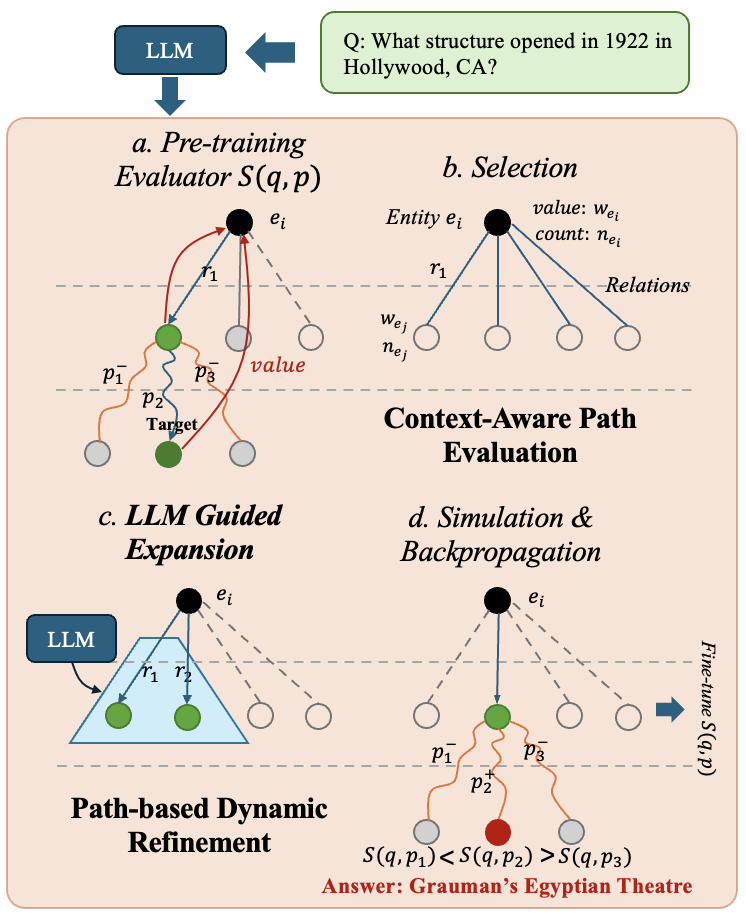
\includegraphics[scale=0.56]{figure/framework.png}
% \vspace{-0.6cm}
\caption{Overview of \method{}. The reasoning process begins with an MCTS guided by an LLM-based planner, which selects top-$k$ semantically relevant relations at each expansion step. A context-aware path evaluator scores each candidate path during simulation. To enable continual adaptation, high-confidence pseudo-paths generated during search are used to dynamically fine-tune the evaluator.}
\label{framework}
\vspace{-1.4cm}
\end{minipage}
\end{wrapfigure}

% \begin{figure}[t!]
%   \centering
%   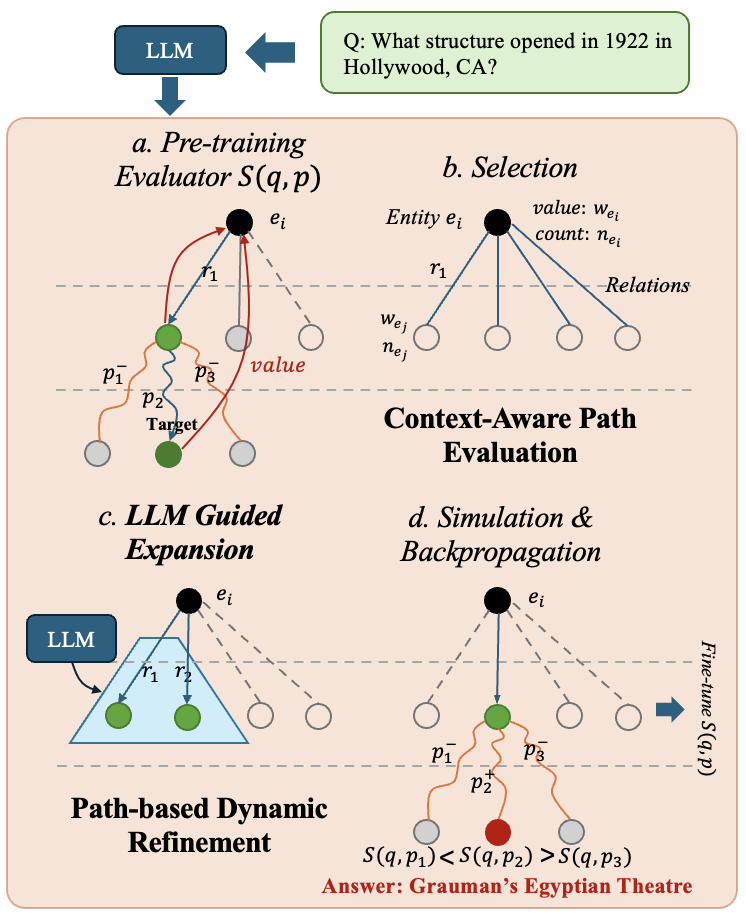
\includegraphics[width=0.48\textwidth]{figure/framework.png} 
%   % \vspace{-0.1cm}
% \caption{Overview of \method{}. The reasoning process begins with an MCTS guided by an LLM-based planner, which selects top-$k$ semantically relevant relations at each expansion step. A context-aware path evaluator scores each candidate path during simulation. To enable continual adaptation, high-confidence pseudo-paths generated during search are used to dynamically fine-tune the evaluator.}
%   \label{framework}
%   % \vspace{-0.4cm}
% \end{figure}

\subsection{Problem Formulation}

We define Knowledge Graph Question Answering (KGQA) as the task of answering a natural language question by reasoning over a knowledge graph (KG). The KG is typically represented as a set of triples $\mathcal{K} = \{(e_s, r, e_o) \} \subseteq \mathcal{E} \times \mathcal{R} \times \mathcal{E}$, where $\mathcal{E}$ and $\mathcal{R}$ denote the sets of entities and binary relations.
The goal of KGQA is to find a set of answers $\mathcal{A}_q \subseteq \{(e_1,r_1,e_2), (e_2,r_2,e_3)\cdots\} $ for question $q$, such that a reasoning path through the KG leads from a topic entity to the correct answer. Formally, this is often framed as mapping $q$ to an executable query program $p_q$, where $\text{LLM}(p_q|{\mathcal{K}}) = \mathcal{A}_q$.

\subsection{Overview of Framework}
In this paper, we propose a dynamically adaptive reasoning framework \method{} for KGQA, as shown in Fig.~\ref{framework}. 
\method{} comprises three components: (1) \textbf{LLM Guided Expansion.} \method{} employs MCTS to incrementally expand reasoning paths, guided by an LLM-based planner that proposes relevant relations. This reduces computational overhead and enhances efficiency in KG exploration; (2) \textbf{Context-Aware Path Evaluation.} To capture the evolving semantics of reasoning paths, \method{} employs a lightweight Transformer-based scorer with cross-attention to jointly encode the question and path embeddings. This enables context-sensitive evaluation and improves the accuracy and relevance of multi-hop reasoning; (3) \textbf{Path-based Dynamic Refinement.} \method{} uses intermediate paths from MCTS as dynamic pseudo-paths to iteratively fine-tune the path evaluator, enhancing its ability to capture question-specific semantics and improving reasoning accuracy.


\subsection{LLM Guided Expansion}

A key challenge in KGQA is efficiently exploring the vast search space of multi-hop reasoning paths, especially under weak or no supervision. Existing methods often struggle to balance search efficiency and semantic relevance, resulting in either redundant exploration or missed correct paths~\citep{long2025enhancing,li2024simple}. To address this, the LLM-Guided Expansion module employs MCTS~\citep{kocsis2006bandit} as the backbone for symbolic path expansion. At each step, an LLM proposes semantically relevant relations, narrowing the search space and improving path quality, while MCTS ensures a balanced trade-off between exploration and exploitation.

% At each step, an LLM-based planner proposes top-$k$ semantically relevant relations based on the current state and the question. MCTS incrementally expands paths and selects promising candidates through simulation and backpropagation, enabling scalable and focused search aligned with the question intent.

% The core of path expansion in \method{} lies in selecting relations relevant to the question $ q $ for further expansion. For reducing computational costs and enhancing efficiency in large-scale knowledge graph exploration, we introduce an LLM-based planner to select the top-k relevant relations for path expansion in the proposed \method{}. 
Specifically, each node in the MCTS represents a reasoning state anchored at a specific entity in the KG. Given the current state, possible actions correspond to selecting an outgoing relation to extend the reasoning path. During the \textbf{Selection} phase, the search traverses from the root to a leaf node by recursively choosing children with the highest Upper Confidence Bound for Trees (UCT) score~\citep{kocsis2006bandit}, which is defined as:
\begin{equation}
\label{selection}
UCT = \frac{w_i}{n_i} + C \sqrt{\frac{\ln N}{n_i}},
\end{equation}
where $w_i$ denotes the accumulated reward of node $i$, $n_i$ its visit count, $N$ the visit count of its parent, and $C$ a constant that balances exploration and exploitation. This criterion guides the search to trade off between exploring new relations and exploiting promising paths.
In the \textbf{Expansion} phase, the selected leaf node is expanded by retrieving the outgoing relations of its entity $e_i$, denoted as $\mathcal{R}_{e_i} = \{r_1, r_2, \dots, r_n\}$. To avoid exhaustive branching, we prompt an LLM with the question $q$ and candidate relations $\mathcal{R}_{e_i}$, selecting the top-$k$ relations most semantically aligned with $q$:
\begin{equation}
\mathcal{R}_{top-k} = \text{LLM}(q, \mathcal{R}_{e_i}).
\end{equation}
These top-$k$ relations are then used to generate new child nodes, ensuring that expansion favors semantically meaningful directions and remains computationally efficient.

% Given a node in the MCTS representing a relation $ r \in \mathcal{R} $, we first retrieve all entities $ e \in \mathcal{E} $ that are connected to this relation $ r $ as the tail entities $ T_r = \{e_1, e_2, \dots, e_n\} $. Then, for each tail entity $ e_i $, we retrieve all relations $ \mathcal{R}_i $ associated with $ e_i $, forming a new set of candidate relations $ \mathcal{R}_{cand} = \bigcup_{e_i \in T_r} \mathcal{R}_i $. These candidate relations are used for expanding the reasoning path. To guide this selection efficiently, we employ an LLM to choose the top-k relations that are most relevant to the question $ q $, based on the current reasoning context. The LLM takes as input the question $ q $ and the set of candidate relations $\mathcal{R}_{cand}$, and outputs the top-k relations $ \mathcal{R}_{top-k} $ most aligned with $ q $:
% \begin{equation}
% \mathcal{R}_{top-k} = \text{LLM}(q, \mathcal{R}_{cand})
% \end{equation}
% This method ensures that only the most relevant relations are considered for path expansion, thereby improving computational efficiency and steering the search toward the correct answer.

\subsection{Context-Aware Path Evaluation}

While LLM-guided expansion effectively narrows the search space by selecting semantically relevant relations, it does not ensure that all expanded paths remain valid in the broader reasoning context. As the search progresses, path semantics evolve dynamically, and early promising trajectories may later become misleading or irrelevant. Prior works attempt to filter or pre-plan paths to improve relevance~\citep{fang2024karpa,long2025eperm}, but still leave gaps in capturing evolving path semantics during search. To address this, we integrate a lightweight Transformer-based path scorer into MCTS’s simulation phase, employing cross-attention to jointly encode the question and current path, enabling adaptive evaluation that reflects evolving semantics.

% While LLM-guided expansion effectively narrows the search space by selecting semantically relevant relations, it cannot guarantee that expanded paths remain valid or meaningful in the broader reasoning context. As the search progresses, path semantics evolve dynamically, and trajectories that appear promising early may later become irrelevant or misleading~\citep{sun2018open,ye2022routing}. To address this, Context-Aware Path Evaluation integrates a lightweight Transformer-based path scorer into the simulation phase of MCTS. This scorer leverages cross-attention to jointly encode the question and the current reasoning path, allowing for adaptive evaluation that captures evolving semantics. By assigning scores to simulated paths based on question-path alignment, this module enables more accurate path ranking throughout the search process.

\textbf{Context-Aware Path Evaluator.} 
In the \textbf{Simulation} phase, we assess the quality of candidate paths generated during MCTS rollouts. Given a question $q$ and a candidate relation path $p_r = (r_1, r_2, \ldots, r_l)$, where $p_r$ is formed by sequentially selecting relations during expansion, both $q$ and $p_r$ are first encoded using a pre-trained LLM. Let $\mathbf{z}_q \in \mathbb{R}^d$ denote the embedding of $q$ and $\mathbf{z}_{r_i} \in \mathbb{R}^d$ the embedding of relation $r_i$. To capture the sequential structure of $p_r$, we introduce a learnable positional encoding $\mathbf{e}_i^{\text{pos}}$ for each relation. The final input sequence is obtained by combining $\mathbf{z}_{r_i}$ with $\mathbf{e}_i^{\text{pos}}$ and feeding the sequence into a Transformer encoder:
\begin{equation}
\mathbf{E}_{p_r} = \text{Transformer}([\mathbf{z}_{r_1} + \mathbf{e}_1^{\text{pos}}, \ldots, \mathbf{z}_{r_l} + \mathbf{e}_l^{\text{pos}}]),
\end{equation}
where $\mathbf{e}_i^{\text{pos}} = \mathbf{E}^{\text{pos}}[i]$ is the positional embedding of the $i$-th hop, drawn from a trainable matrix $\mathbf{E}^{\text{pos}} \in \mathbb{R}^{L \times d}$, where $L$ is the maximum path length and $d$ the embedding dimension. To further incorporate question-specific information, we apply a cross-attention mechanism, allowing the encoded path representation $\mathbf{e}_{p_r}$ to attend to the question embedding $\mathbf{z}_q$:
\begin{equation}
\mathbf{H} = \mathbf{E}_{p_r} + \mathrm{CrossAttn}(\mathbf{E}_{p_r}, \mathbf{z}_q),    \;
% \end{equation}
% \begin{equation}
    with\; \text{CrossAttn}(\mathbf{E}_{p_r}, \mathbf{z}_q)=\text{softmax}({\mathbf{E}_{p_r} \cdot \mathbf{z}_q^T}/{\sqrt{d_k}}) \cdot \mathbf{z}_q. 
\end{equation}
We then apply attention pooling over the relation representations $\mathbf{H}$ to obtain the hidden state of the relation path:
\begin{equation}
\mathbf{s}_{p_r} = \sum_{i=1}^l \alpha_i \textbf{h}_i, \quad \alpha = \text{Softmax}\big(\text{MLP}(\mathbf{H})\big),    
\end{equation}
where $\mathbf{h}_i$ is the hidden state of the $i$-th relation and $\alpha_i$ its learned attention weight. This pooling allows the model to emphasize informative steps along the reasoning path. The pooled path representation $\mathbf{s}_{p_r}$ is then concatenated with the question embedding $\mathbf{z}_q$, and the combined vector is passed through a multi-layer perceptron to compute the plausibility score of the question–path pair:
\begin{equation}
S(q, p_r) = \mathrm{MLP}\big([\mathbf{s}_{p_r}:\mathbf{z}_q]\big).    
\end{equation}
This context-aware evaluator assigns plausibility scores to partial reasoning paths by jointly encoding the question and relation sequence, providing accurate, context-sensitive guidance for MCTS.
% This context-aware evaluation model dynamically scores partial reasoning paths by jointly considering the question and the relation sequence, offering accurate and context-sensitive guidance to the MCTS search process.


\textbf{Pre-training of Evaluator.} To train the context-aware evaluator, we construct supervision by sampling positive and negative paths from local subgraphs. A path is positive if it links the head entity to a correct answer within a hop limit. Negatives come from two sources: hard negatives that terminate near but miss the answer, and random negatives from walks that avoid answer entities. Each training instance is a triplet $(q, p^+, p^-)$, with sequences zero-padded and masked for efficient batch training.

The model computes a plausibility score $S(q, p)$ for each question-path pair and is optimized using the Pair-wise Ranking loss~\citep{rendle2012bpr} to encourage higher scores for positive paths:
\begin{equation}
\label{pr}
    \mathcal{L}_{\text{PR}} = -\frac{1}{M} \sum_{i=1}^M \log \sigma\left( S(q, p^+_i) - S(q, p^-_i) \right),
\end{equation}
where $\sigma(\cdot)$ is the sigmoid function. This training strategy equips the evaluator with the ability to distinguish plausible reasoning paths, thereby improving the guidance signal during MCTS inference.
% Each training instance consists of a triplet $(q, p^+, p^-)$, where $p^+$ and $p^-$ are the positive and negative relation sequences, respectively. All relation sequences are zero-padded to a fixed maximum length $L$, and binary masks are generated to support efficient batch training. 

% Given a question-path pair $(q, p)$, let $S(q, p)$ denote the plausibility score computed by the evaluation model. The model is trained to discriminate positive paths from negative ones by minimizing the Bayesian Personalized Ranking (BPR) loss:
% \begin{equation}
% \mathcal{L}_{\text{BPR}} = -\frac{1}{N} \sum_{i=1}^N \log \sigma\left( S(q, p^+_i) - S(q, p^-_i) \right),    
% \end{equation}
% where $\sigma(\cdot)$ is the sigmoid function and $N$ is the batch size.

% To promote stable and effective learning, we ensure data deduplication for unique path sequences, dynamically balance the number of positive and negative samples, and utilize attention masking for variable-length paths during batch processing. This comprehensive training paradigm equips the model with the capacity to distinguish plausible reasoning paths from implausible ones, thereby providing a robust foundation for accurate and context-sensitive path evaluation during the search process.




\subsection{Path-based Dynamic Refinement}

While LLM-guided expansion and semantic scoring improve path exploration, the static evaluator may fail to generalize to the evolving search space. To address this, we introduce a dynamic refinement mechanism that leverages high-confidence paths from MCTS rollouts as pseudo-paths. 
These pseudo-paths serve as supervision signals, enabling continual adaptation of the evaluator to new reasoning contexts without requiring additional labeled data.
% These are used to incrementally fine-tune the evaluator, enabling it to adapt to new reasoning contexts and improve path selection without relying on additional supervision.

Specifically, during \textbf{Backpropagation} phase, the plausibility score estimated by the context-aware path evaluator is propagated along the visited nodes in the MCTS tree after each simulation. For every entity $e_i$ on the simulated path, we update its visit count and aggregated value as follows:
\begin{equation}
    n_{e_i}= n_{e_i} + 1, \quad w_{e_i}= \frac{\sum_j n_{e_j}\cdot w_{e_j}}{\sum_j n_{e_j}},
\end{equation}
where $n_{e_i}$ is the visit count and $w_{e_i}$ is the aggregated value of entity $e_i$. The value is computed as a weighted average over its child nodes $\{e_j\}$, and reflects the plausibility scores $w_{e_j}$ assigned during simulation. These updates refine the UCT estimates used in future selection steps, progressively biasing the search toward high-quality reasoning paths.

To construct supervision signals for fine-tuning, we dynamically sample pseudo-path pairs ($\hat{p}'_i$, $\hat{p}'_j$) from the set of explored paths during MCTS. Instead of relying on the evaluator’s predictions, we assign pseudo-labels based on empirically grounded values derived from the search process. Specifically, for entity $e_i$ along a reasoning path $p_r$, we define its search value as:
$w_{e_i} = \frac{w_{p_r}}{n_{e_i}}$,
where $w_{p_r}$ is the cumulative reward from all rollouts passing through $p_r$, and $n_{e_i}$ is the visite count of entity $e_i$.
Given a pair of paths, we assign pseudo-labels based on their relative values:
\begin{equation}
    \left(\hat{p}^+,\, \hat{p}^-\right) =
\begin{cases}
(p'_i,\, p'_j), & \text{if } w_{e_i} > w_{e_j}, \\
(p'_j,\, p'_i), & \text{otherwise}.
\end{cases}
\end{equation}
The path evaluator is then fine-tuned using the Pair-wise Ranking loss in Eq.~\ref{pr}, encouraging higher scores for more promising paths.






% This refinement process is periodically triggered during MCTS rollouts, allowing the evaluation model to adapt to the evolving search space. By leveraging search-derived feedback, the model continuously improves its ability to distinguish between effective and ineffective reasoning paths, enhancing search efficiency, model robustness, and generalization across diverse KGQA scenarios.
% To further enhance the adaptability and effectiveness of the path evaluation model, we introduce a dynamic pseudo-path refinement strategy seamlessly integrated within the MCTS framework. 


% To construct high-quality supervision signals for fine-tuning the path evaluation model, we first dynamically sample pairs of pseudo paths $(\hat{p}'_i, \hat{p}'_j)$ from the set of explored paths. Crucially, instead of relying on the model's direct score, we leverage the empirically grounded values derived from the MCTS search process itself. For each explored path p (represented as a node in the tree), we define its MCTS value $V_{MCTS}(p) = \frac{p.value}{p.counts}$ as the ratio of its total accumulated rewards to its visit count, where p.value denotes the sum of outcomes from all simulations that have passed through it, and p.visits denotes the total number of times that node has been visited during the MCTS search process. For each pair, we use
% and assign positive and negative labels as follows:
% \begin{equation}
% \left(\hat{p}^+,\, \hat{p}^-\right) =
% \begin{cases}
%     (p'_i,\, p'_j), & \text{if}\;\; V_{MCTS}(p'_i) > V_{MCTS}(p'_j) \\
%     (p'_j,\, p'_i). & \text{otherwise}
% \end{cases}
% \end{equation}
% Then, we also use the optimization objective in Eq.(6) to fine-tune the path evaluation model, encouraging it to assign higher plausibility scores to more promising reasoning paths. 

% This pseudo-label refinement process is invoked periodically throughout the MCTS search, typically after a sufficient number of search iterations, allowing the evaluation model to adapt to the dynamically evolving distribution of explored paths. By grounding the training process in feedback derived directly from ongoing search trajectories, the model is continuously updated and aligned with the current reasoning context. This dynamic self-improvement mechanism enables the framework to more reliably discriminate between effective and ineffective reasoning paths, resulting in improved search efficiency, enhanced model robustness, and superior generalization performance across diverse knowledge graph environments.

\subsection{Reasoning Process}

The overall reasoning process is outlined in Appendix~\ref{sec:algorithm}. The framework first initializes a path evaluator to discriminate between plausible and implausible KG paths, providing a foundation for downstream search. During dynamic MCTS, the algorithm iteratively performs selection, expansion, simulation, and backpropagation. In expansion, an LLM-based planner adaptively selects the top-$k$ relations most relevant to the question, steering the search toward semantically meaningful paths. The evaluator guides simulation by prioritizing trajectories likely to yield correct answers, while pseudo-path pairs sampled during search are periodically used for refinement. Finally, entities reached by high-scoring paths are aggregated to form the answer set.





\section{Experiments}




\subsection{Experimental Settings}
\textbf{Datasets.} {To evaluate the effectiveness of \method{}, we conduct experiments on two widely used KGQA benchmarks: WebQSP~\cite{talmor2018web} and CWQ~\cite{yih2016value}. Following prior work~\cite{sun2023think,liu2025dual}, we uniformly sample 1,000 questions from the test sets of both datasets to evaluate the performance.} More details about datasets are provided in Appendix ~\ref{sec:dataset}. 



\noindent\textbf{Baselines.} We compare \method{} with a comprehensive set of baselines. These baselines include: the semantic parsing methods, e.g., KV-Mem~\citep{miller2016key}, EmbedKGQA~\citep{saxena2020improving}, QGG~\citep{lan2020query}, NSM~\citep{he2021improving}, TransferNet~\citep{shi2021transfernet}, and KGT5~\citep{saxena2022sequence};
the retrieval-based methods, e.g., GraftNet~\citep{sun2018open}, PullNet~\citep{sun2019pullnet}, SR+NSM~\citep{zhang2022subgraph}, and SR+NSM+E2E~\citep{zhang2022subgraph};
the general LLMs, including 
Flan-T5-xl~\citep{chung2024scaling}, Alpaca-7B~\citep{taori2023stanford},
Llama3-8B~\citep{dubey2024llama}, Qwen2.5-7B~\citep{team2024qwen2}, ChatGPT~\citep{schulman2022chatgpt}, and ChatGPT+CoT~\citep{wei2022chain};
and recent LLMs with KG methods, including UniKGQA~\citep{jiang2022unikgqa},DECAF~\citep{yu2022decaf}, KD-CoT~\citep{wang2023knowledge},
Nutrea~\citep{choi2023nutrea}, ToG~\citep{sun2023think}, RoG~\citep{luo2023reasoning}, KAPING~\citep{baek2023knowledge}, ReasoningLM~\citep{jiang2023reasoninglm},
FiDeLis~\citep{sui2024fidelis}, GNN-RAG~\citep{mavromatis2024gnn},
DoG~\citep{ma2025debate},  DualR~\citep{liu2025dual}
, DP~\citep{ma2025deliberation}, and RwT~\citep{shen2025reasoning}. The details are provided in Appendix~\ref{sec:baseline}.

% \noindent\textbf{Evaluation Metric.} Following~\citep{luo2023reasoning,yao2025learning,ma2025deliberation}, we evaluate \method{} using Hits@1 and F1 score, assessing answer correctness and overall accuracy for questions with potentially multiple correct answers.
\begin{table*}[t]
\centering
\small
\begin{tabular}{clcccc}
\toprule
\multirow{2}{*}{\textbf{Type}} 
& \multirow{2}{*}{\textbf{Methods}} 
& \multicolumn{2}{c}{\textbf{WebQSP}} 
& \multicolumn{2}{c}{\textbf{CWQ}} \\
& & Hits@1 & F1 & Hits@1 & F1 \\
\midrule
\multirow{6}{*}{Semantic Parsing} 
& KV-Mem~\citep{miller2016key} & 46.7 & 34.5 & 18.4 & 15.7 \\
& EmbedKGQA~\citep{saxena2020improving} & 66.6 & - & 45.9 & - \\
& QGG~\citep{lan2020query} & 73.0 & 73.8 & 36.9 & 37.4 \\
& NSM~\citep{he2021improving} & 68.7 & 62.8 & 47.6 & 42.4 \\
& TransferNet~\citep{shi2021transfernet} & 71.4 & - & 48.6 & - \\
& KGT5~\citep{saxena2022sequence} & 56.1 & - & 36.5 & - \\
\midrule
\multirow{4}{*}{Retrieval} 
& GraftNet~\citep{sun2018open} & 66.4 & 60.4 & 36.8 & 32.7 \\
& PullNet~\citep{sun2019pullnet} & 68.1 & - & 45.9 & - \\
& SR+NSM~\citep{zhang2022subgraph} & 68.9 & 64.1 & 50.2 & 47.1 \\
& SR+NSM+E2E~\citep{zhang2022subgraph} & 69.5 & 64.1 & 49.3 & 46.3 \\
\midrule
\multirow{6}{*}{LLMs} 
& Flan-T5-xl~\cite{chung2024scaling} & 31.0 & - & 14.7 & - \\
& Alpaca-7B~\cite{taori2023stanford} & 51.8 & - & 27.4 & - \\
& Llama3-8B~\citep{dubey2024llama} & 30.3 & 25.7 & 30.5 & 27.8 \\
& Qwen2.5-7B~\citep{team2024qwen2} & 28.4 & 23.7 & 25.9 & 24.1 \\
& ChatGPT~\citep{schulman2022chatgpt} & 66.8 & - & 39.9 & - \\
& ChatGPT+CoT~\citep{wei2022chain} & 75.6 & - & 48.9 & - \\
\midrule
\multirow{13}{*}{LLMs+KGs} 
& UniKGQA~\citep{jiang2022unikgqa} & 77.2 & 72.2 & 51.2 & 49.0 \\
& DECAF~\cite{yu2022decaf} & 82.1 & 78.8 & 70.4 & - \\
& KD-CoT~\cite{wang2023knowledge} & 68.6 & 52.5 & 55.7 & - \\
& Nutrea~\citep{choi2023nutrea} & 77.4 & 72.7 & 53.6 & 49.5 \\
& ToG~\citep{sun2023think} & 81.9 & 76.0 & 68.5 & 60.2 \\
& RoG~\citep{luo2023reasoning} & 80.8 & 70.8 & 57.8 & 56.2 \\
& KAPING~\citep{baek2023knowledge} & 72.4 & 65.1 & 53.4 & 50.3 \\
& ReasoningLM~\citep{jiang2023reasoninglm} & 78.5 & 71.0 & 69.0 & 64.0 \\
& FiDeLis~\citep{sui2024fidelis} & 84.3 & 78.3 & 71.5 & 64.3 \\
& GNN-RAG~\citep{mavromatis2024gnn} & 82.8 & 73.5 & 62.8 & 60.4 \\
& DoG~\citep{ma2025debate} & 65.4 & 55.6 & 41.0 & 46.4 \\
& DualR~\citep{liu2025dual} & 81.5 & 71.6 & 65.3 & 62.1 \\
& DP~\citep{ma2025deliberation} & {87.5} & {81.4} & {75.8} & {69.4} \\
& RwT~\citep{shen2025reasoning} & 87.0 & 79.7 & 72.4 & 66.7 \\
\midrule
& \method{} & \textbf{94.0} & \textbf{81.7} & \textbf{78.0} & \textbf{75.1} \\
\bottomrule
\end{tabular}
\vspace{-2pt}
\caption{Performance comparison (\%) on WebQSP and CWQ datasets. \textbf{Bold} results indicate the best performance.}

\label{tab:main_results}
\end{table*}

\noindent\textbf{Implementation Details.} We implement the DAMR framework using PyTorch, and all experiments are conducted on NVIDIA A100 GPUs. The LLM-based planner is implemented with GPT-4.1~\citep{liu2023evaluating}, while question and relation embeddings are generated from Qwen3-Embedding-8B~\citep{yang2025qwen3} with an embedding dimension of 1024. For the path evaluation module, we use a 128-dimensional embedding and employ the Adam optimizer~\citep{kingma2014adam} with a learning rate of $1\times10^{-4}$ during pretraining and $1 \times 10^{-5}$ during fine-tuning. The model consists of two Transformer layers and is trained for 15 epochs in the pretraining stage and 10 epochs in the fine-tuning stage. Following~\citep{luo2023reasoning,yao2025learning,ma2025deliberation}, we evaluate \method{} using Hits@1 and F1 score, assessing answer correctness and overall accuracy for questions with potentially multiple correct answers.



\subsection{Performance Comparison}

We report the experimental results of \method{} in Table~\ref{tab:main_results}, benchmarking its performance against state-of-the-art baselines across KGQA datasets. From the results, we find that: 
% (1) Semantic parsing and retrieval-based methods provide a foundational backbone for KGQA by capturing structural semantics and retrieving relevant subgraphs from large-scale knowledge bases. While embedding-based models encode entity and relation representations, they often fall short in modeling complex relational dependencies and multi-hop reasoning patterns. Retrieval-based approaches offer richer contextual signals through explicit subgraph construction, enhancing reasoning over relevant neighborhoods. However, their dependence on pre-defined retrieval pipelines restricts adaptability to evolving query semantics. 
(1) Semantic parsing and retrieval-based methods serve as early foundations for KGQA by extracting subgraphs and capturing structural semantics. However, embedding-based models struggle with complex relational patterns, while retrieval-based methods rely on rigid pipelines that limit generalization. In contrast, LLM with KG approaches combine the language understanding of LLMs with structured reasoning over KGs, enabling more flexible path exploration and improved adaptability to diverse, multi-hop queries.
(2) General-purpose LLMs, such as ChatGPT and Llama3-8B, show basic reasoning ability but often perform worse than methods that combine LLMs with KGs in KGQA tasks. This is mainly because they are not grounded in domain-specific knowledge, making them more likely to produce incorrect or made-up answers. 
% (2) LLMs with KG methods significantly enhance reasoning effectiveness by integrating LLMs and structured relational knowledge. The inclusion of graph-based entity and relation embeddings enables these methods to capture richer semantic relationships and more effectively handle complex multi-hop queries. Consequently, these methods approaches consistently outperform general LLMs across both datasets. 
(3) \method{} consistently outperforms all baselines across both datasets, showcasing its strong reasoning capability. This superior performance is driven by its integration of an LLM-based planner, which selectively retrieves relevant relations to reduce noise and guide the search toward high-quality reasoning paths, and a path evaluation model that is dynamically fine-tuned during search to capture semantic differences among candidate paths and accurately rank those most likely to yield correct answers.


\vspace{-1pt}
\subsection{Efficiency Analysis}
As shown in Table~\ref{tab:Efficiency}, \method{} achieves substantial improvements in computational efficiency. It reduces the average number of LLM calls to 7.1 on WebQSP and 16.8 on CWQ, with corresponding token usage of 3,931 and 9,266. These correspond to reductions of over 50\% in LLM calls and 75\% in token consumption relative to the strongest baseline. This efficiency is achieved by invoking the LLM only during the expansion phase of MCTS to select the top-$k$ semantically relevant relations, which effectively narrows the search space and avoids redundant reasoning steps that lead to unnecessary computational overhead. During simulation, the context-aware path evaluator efficiently assesses candidate paths based on question-path alignment without requiring any further LLM interaction or model inference. These design choices reduce both the frequency and verbosity of LLM usage while maintaining strong reasoning performance, making \method{} more efficient, scalable, and practically deployable than previous work.

% To assess the computational efficiency of \method{}, we evaluate its average number of LLM calls and token consumption per question on the WebQSP and CWQ datasets. As shown in Table~\ref{tab:Efficiency}, \method{} significantly reduces both LLM calls and token usage compared to baselines such as DoG~\citep{ma2025debate}, ToG~\citep{luo2023reasoning}, and RwT~\citep{shen2025reasoning}. Specifically, \method{} lowers the average number of LLM calls to 7.1 on WebQSP and 16.8 on CWQ, achieving over a 50\% reduction relative to the most efficient baseline. Similarly, it reduces token consumption by more than 75\% on both datasets. These results demonstrate the superior efficiency of \method{}, making it considerably more practical and cost-effective for real-world deployment.



\subsection{Ablation Study}\label{sec:ablation}

We conduct ablation studies to assess the contributions of key components in \method{}: (1) \method{} w/o PE: removing the path evaluation module; (2) \method{} w/o FT: disabling fine-tuning of the evaluator; and (3) \method{} w/ GPT-4.1: replacing the context-aware evaluator with a general LLM.

Experimental results are summarized in Table~\ref{tab:ablation_results}. From the results, we find that:
(1) Removing the path evaluation module (\method{} w/o PE) causes a noticeable performance drop on both datasets, underscoring its critical role in guiding the search process. Without this component, the model cannot effectively assess or rank candidate paths, leading to suboptimal reasoning and reduced accuracy.
(2) Compared to \method{} w/o FT, the proposed \method{} consistently achieves superior results on both datasets, highlighting the importance of the finetuning mechanism in the path evaluation module. This mechanism enables the model to adapt to the evolving distribution of explored paths, improving its ability to distinguish plausible from implausible reasoning trajectories.
(3) Replacing the context-aware path evaluation module with general LLMs yields degraded performance, confirming the advantage of our fine-tuned path scorer. By capturing fine-grained semantic distinctions among candidate paths, it provides more accurate evaluation signals, enhancing overall search effectiveness.

% \begin{table}[t]
% \centering
% \small
% \begin{tabular}{l|cc|cc}
% \toprule
% \multirow{2}{*}{Method} & \multicolumn{2}{c}{WebQSP} & \multicolumn{2}{c}{CWQ} \\
%  & Hits@1 & F1 & Hits@1 & F1 \\
% \midrule

% \method{} w/o PE & 91.2 & 78.2 & 74.3 & 72.1 \\

% \method{} w/o FT & 91.9 & 80.1 & 75.1 & 73.0 \\

% \method{} w/ GPT 4.1 & 92.5 & 79.8 & 74.9 & 72.4 \\

% % \method{} w GPT 4.1-mini & 92.9 & 80.1 & 75.4 & 72.8 \\

% % \method{} w Llama2-13B & 92.0 & 78.8 & 75.2 & 72.5 \\

% % \method{} w Qwen3-14B & 92.3 & 79.2 & 75.7 & 73.3 \\

% \midrule

% \method{} & \textbf{94.0} & \textbf{81.7} & \textbf{78.0} & \textbf{75.1} \\

% \bottomrule
% \end{tabular}
% \caption{The results of ablation studies on the WebQSP and CWQ datasets. \textbf{Bold} results indicate the best performance.}
% \label{tab:ablation_results}
% \end{table}

\begin{table}[t]
\centering
\begin{minipage}{\textwidth}
\begin{minipage}[t]{0.47\textwidth}
\makeatletter\def\@captype{table}
\centering
\footnotesize
\tabcolsep=3pt
\begin{tabular}{l@{\hspace{2em}}|cc|cc}
\toprule
\multirow{2}{*}{Method} & \multicolumn{2}{c|}{WebQSP} & \multicolumn{2}{c}{CWQ} \\
 & \#Tokens & \#Calls & \#Tokens & \#Calls \\
\midrule
DoG       & 22,538 & 30.9  & 37,741 & 58.1 \\
ToG       & 16,372 &  23.2 & 26,183 & 41.9 \\
RwT       & 10,680 & 15.1 & 17,885 &  28.6 \\
\midrule
\method{} &  \textbf{3,931} & \textbf{7.1} &  \textbf{9,266} &  \textbf{16.8} \\
\bottomrule
\end{tabular}
\vspace{0.5cm}
\caption{Statistics of average number of LLM calls and token consumption per question on WebQSP and CWQ datasets.}
\label{tab:Efficiency}
\end{minipage}
\hspace{0.18in}
\begin{minipage}[t]{0.48\textwidth}
\makeatletter\def\@captype{table}
\centering
\footnotesize
\tabcolsep=3pt
\begin{tabular}{l|cc|cc}
\toprule
\multirow{2}{*}{Method} & \multicolumn{2}{c}{WebQSP} & \multicolumn{2}{c}{CWQ} \\
 & Hits@1 & F1 & Hits@1 & F1 \\
\midrule

\method{} w/o PE & 91.2 & 78.2 & 74.3 & 72.1 \\

\method{} w/o FT & 91.9 & 80.1 & 75.1 & 73.0 \\

\method{} w/ GPT 4.1 & 92.5 & 79.8 & 74.9 & 72.4 \\

% \method{} w GPT 4.1-mini & 92.9 & 80.1 & 75.4 & 72.8 \\

% \method{} w Llama2-13B & 92.0 & 78.8 & 75.2 & 72.5 \\

% \method{} w Qwen3-14B & 92.3 & 79.2 & 75.7 & 73.3 \\

\midrule

\method{} & \textbf{94.0} & \textbf{81.7} & \textbf{78.0} & \textbf{75.1} \\

\bottomrule
\end{tabular}
\vspace{0.5cm}
\caption{The results of ablation studies on the WebQSP and CWQ datasets. \textbf{Bold} results indicate the best performance.}
\label{tab:ablation_results}
\end{minipage}
\end{minipage}
\vspace{-0.5cm}
\end{table}


\begin{wrapfigure}{r}{0.6\textwidth}
\vspace{-0.9cm}
\begin{minipage}[t]{0.6\textwidth}
        \centering
        \hspace{-1cm}
    \subfloat[Number of selected relations $k$]{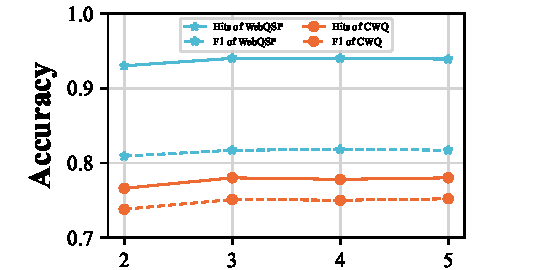
\includegraphics[width=0.53\textwidth,height=0.29\textwidth]{figure/hyper_top_k.pdf}}
    \label{fig:mcts_top_k}
    \hspace{-0.5cm}
    \subfloat[Reasoning path length $L$]{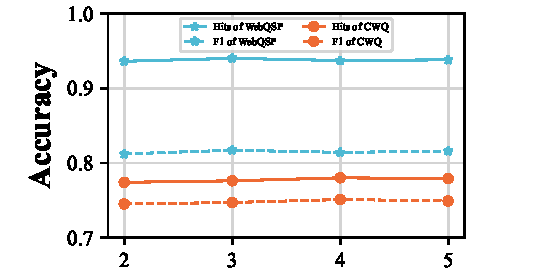
\includegraphics[width=0.53\textwidth,height=0.29\textwidth]{figure/hyper_mcts_deep.pdf}}
    \label{fig:mcts_length}
    \hspace{-1.3cm}
    \vspace{-0.2cm}
    \caption{Sensitivity analysis of hyperparameter on the WebQSP and CWQ datasets.}
        \label{fig:hyper_sensitive}
    \end{minipage}%
    \vspace{-0.4cm}
\end{wrapfigure}


\subsection{Sensitivity Analysis}\label{sec:sensitivity}

We conduct a sensitivity analysis to assess the impact of two key hyperparameters in \method{}: the number of selected relations $k$ and the maximum reasoning path length $L$. The parameter $k$ controls how many relations are proposed by the LLM-based planner at each step, while $L$ determines the number of reasoning hops allowed during path construction.

Figure \ref{fig:hyper_sensitive} illustrates how $k$ and  $L$ affect the performance of \method{} on the WebQSP and CWQ datasets. We vary $k$ and $L$ within the range of  $\{2, 3, 4, 5\}$. From the results, we observe that: (1) As shown in Figure~\ref{fig:hyper_sensitive}(a), increasing $k$ initially leads to performance gains, which then stabilize before experiencing a slight decline. While larger $k$ values encourage broader relational exploration, they may also introduce irrelevant candidates and increased computational cost. Conversely, smaller $k$ restrict the diversity of the search. To balance these trade-offs, we select a moderate $k=3$ as the default setting. (2) As shown in Figure~\ref{fig:hyper_sensitive}(b), on the WebQSP dataset, performance improves from $L=2$ to $3$, then fluctuates between $L=3$ and $5$, suggesting limited gains beyond three hops. In contrast, performance on the CWQ dataset steadily increases up to $L=4$ before slightly declining at $L=5$, reflecting its need for deeper reasoning due to more complex questions. Balancing effectiveness and efficiency across both datasets, we set $L=4$ as the default path length in all experiments. 
More results are provided in Appendix ~\ref{sec:experiments_results}.





% \vspace{-5pt}
\subsection{Impact of Different LLMs} 
\begin{wraptable}{r}{0.6\textwidth} 
\vspace{-29pt}
\footnotesize
\centering
\tabcolsep=6pt
\begin{tabular}{l|cc|cc}
\toprule
\multirow{2}{*}{Method} & \multicolumn{2}{c}{WebQSP} & \multicolumn{2}{c}{CWQ} \\
 & Hits@1 & F1 & Hits@1 & F1 \\
\midrule
\method{} (Llama2-13B) & 91.0 & 76.7 & 73.9 & 69.5 \\
\method{} (Qwen3-14B) & 91.5 & 77.8 & 74.4 & 70.1 \\
\method{} (GPT 4.1-mini) & 93.1 & 80.6 & 76.1 & 72.7 \\
\method{} (GPT 4.1) & \textbf{94.0} & \textbf{81.7} & \textbf{78.0} & \textbf{75.1} \\
\bottomrule
\end{tabular}
            % \caption{Example Table}
            \caption{Performance of \method{} using different LLM-based planners as backbones on different datasets.}\label{tab:backbone_results}
\end{wraptable}
To evaluate the impact of different LLM-based planners within the \method{} framework, we compare several backbones including Llama2-13B~\citep{roque2025evolution}, Qwen3-14B~\citep{team2024qwen2}, GPT 4.1 mini, and GPT 4.1, as shown in Table~\ref{tab:backbone_results}. Across both datasets, stronger LLMs consistently yield higher F1 and Hits scores, with GPT 4.1 achieving the best performance across all metrics. These results highlight the pivotal role of advanced LLMs in guiding relation selection and reasoning path expansion, where improved fluency, contextual awareness, and semantic precision translate into more accurate and faithful reasoning trajectories. Notably, the consistent performance gap between smaller and larger backbones illustrates the sensitivity of KGQA systems to the planner’s reasoning capability, reinforcing the necessity of leveraging high-capacity models when available. Overall, these findings emphasize the importance of backbone selection and further validate the design of \method{}, which capitalizes on powerful LLMs to achieve robust, generalizable, and effective multi-hop reasoning.

% \begin{figure*}[t]
%     \centering
%     % 左侧：图片
%     \begin{minipage}[t]{0.48\textwidth}
%         \centering
%         \hspace{-1cm}
%     \subfloat[Number of selected relations $k$]{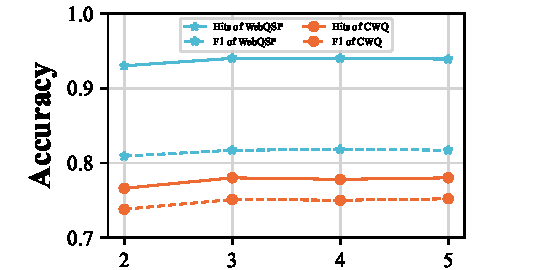
\includegraphics[width=0.53\textwidth,height=0.29\textwidth]{figure/hyper_top_k.pdf}}
%     \label{fig:mcts_top_k}
%     \hspace{-0.5cm}
%     \subfloat[Reasoning path length $L$]{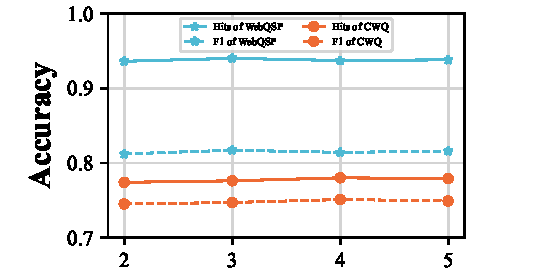
\includegraphics[width=0.53\textwidth,height=0.29\textwidth]{figure/hyper_mcts_deep.pdf}}
%     \label{fig:mcts_length}
%     \hspace{-1.3cm}

%     \caption{ Sensitivity analysis of hyperparameter on the WebQSP and CWQ datasets.}
%         \label{fig:hyper_sensitive}
%     \end{minipage}%
%     \hfill
%     % 右侧：表格
%     \begin{minipage}[t]{0.48\textwidth}
%     \vspace{-2.9cm}
%         \centering
        
%         \begin{table}[H] % 使用 [H] 防止表格浮动，需 \usepackage{float}
%             \centering
%             \small
%             % \setlength{\tabcolsep}{7pt}
% \begin{tabular}{l|cc|cc}
% \toprule
% \footnotesize
% \tabcolsep=5pt
% \multirow{2}{*}{Method} & \multicolumn{2}{c}{WebQSP} & \multicolumn{2}{c}{CWQ} \\
%  & Hits@1 & F1 & Hits@1 & F1 \\
% \midrule

% \method{} (Llama2-13B) & 91.0 & 76.7 & 73.9 & 69.5 \\

% \method{} (Qwen3-14B) & 91.5 & 77.8 & 74.4 & 70.1 \\

% \method{} (GPT 4.1-mini) & 93.1 & 80.6 & 76.1 & 72.7 \\

% \method{} (GPT 4.1) & \textbf{94.0} & \textbf{81.7} & \textbf{78.0} & \textbf{75.1} \\

% \bottomrule
% \end{tabular}
%             % \caption{Example Table}
%             \caption{Performance of \method{} using different LLM-based planners as backbones on the WebQSP and CWQ datasets. \textbf{Bold} values denote the best results.}\label{tab:backbone_results}
%         \end{table}
%     \end{minipage}
% \end{figure*}


% \begin{table*}[t]
% \renewcommand{\arraystretch}{1.3}
% \small
% \centering
% % \vspace{-0.1cm}
% \begin{tabular}{>{\centering\arraybackslash}m{2.5cm}|p{7.6cm}}
% \toprule
% \textbf{Question} & What structure opened in 1922 in Hollywood, CA? \\
% \hline
% \textbf{Answer} & \textcolor{red}{Grauman's Egyptian Theatre} \\
% \hline
% \multirow{4}{*}{\textbf{Llama-2-13B}} & \textcolor{blue}{The Grauman's Chinese Theatre}, a historic movie palace, opened on November 18, 1922, in Hollywood, CA. It was built by Sid Grauman and Charles E. Toberman and has since become a famous landmark and tourist attraction. \\
% \hline
% \multirow{4}{*}{\textbf{Qwen-3-14B}} & \textcolor{blue}{The TCL Chinese Theatre}, originally known as the Chinese Grand Theatre, opened in 1922 in Hollywood, CA. It is a historic movie theater renowned for its unique architecture and celebrity handprints and footprints. \\
% \hline
% \multirow{3}{*}{\textbf{GPT 4.1}} & \textcolor{blue}{The Hollywood Bowl}, an iconic amphitheater in Hollywood, California, opened in 1922. It is renowned for its distinctive band shell and has hosted numerous concerts and events, becoming a significant cultural landmark in the area. \\
% \hline
% \multirow{3}{*}{\textbf{GPT 4.1-mini}} & \textcolor{blue}{The Hollywood Bowl}, an iconic amphitheater in Hollywood, California, opened in 1922 and has since been a renowned venue for music performances and cultural events. \\
% \hline
% \multirow{7}{*}{\textbf{\method{}}} & \texttt{Path 1}: Entity (id: 83076) $\rightarrow$ location.location.events $\rightarrow$ time.event.locations $\rightarrow$ travel.travel\_destination.tourist\_attractions $\rightarrow$ \textcolor{red}{Grauman's Egyptian Theatre}.  

% \texttt{Path 2}: Entity (id: 83076) $\rightarrow$ travel.travel\_destination.tourist\_attractions $\rightarrow$ \textcolor{red}{Grauman's Egyptian Theatre}. \\
% \bottomrule
% \end{tabular}
% \caption{Case study of \method{}. We highlight the correct answers in \textcolor{red}{Red} and the wrong answers in \textcolor{blue}{Blue}.}
% \label{tab:case_study_method}
% \vspace{-0.4cm}
% \end{table*}


\begin{figure}[t]
    \centering
    \subfloat[One example from the WebQSP dataset.]{
    \label{fig:webqsp}    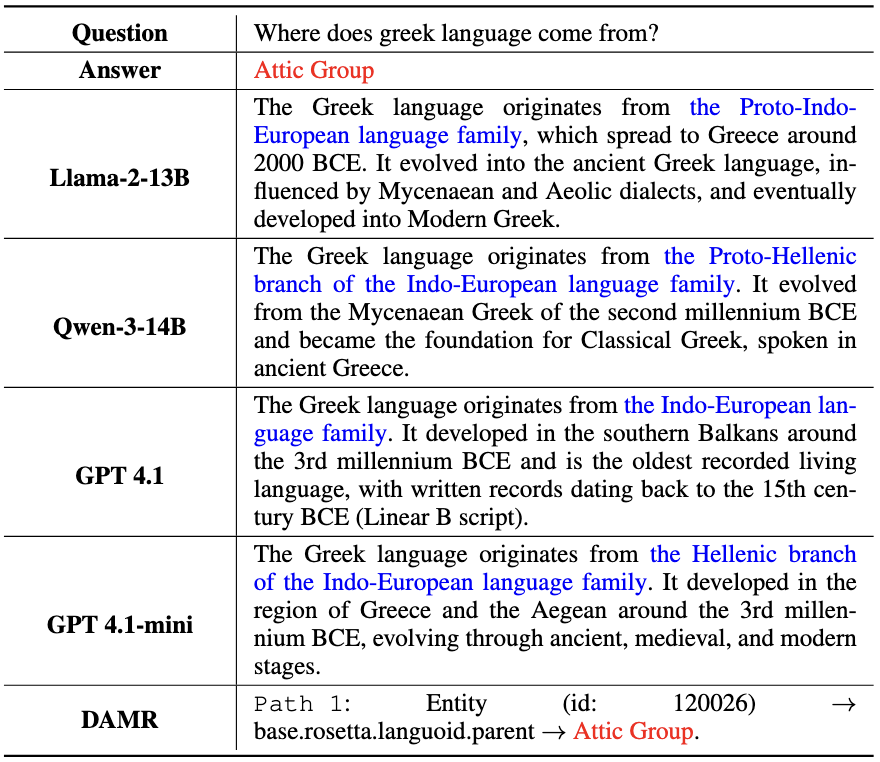
\includegraphics[width=0.47\linewidth]{figure/case_study_1.png}
    }
    \hspace{0.02\linewidth}
    \subfloat[One example from the CWQ dataset.]{
        \label{fig:cwq} 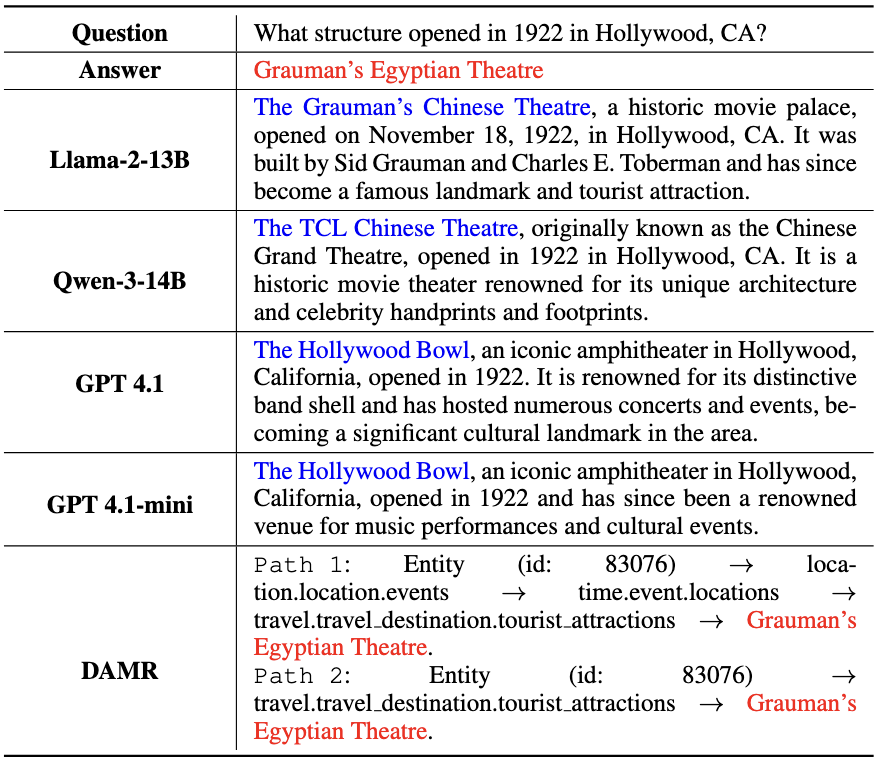
\includegraphics[width=0.47\linewidth]{figure/case_study_2.png}
    }
    \caption{Case studies of \method{} on the WebQSP and CWQ datasets. We highlight the correct answers in \textcolor{red}{Red} and the wrong answers in \textcolor{blue}{Blue}.}
    \label{fig:two_side_by_side}
\end{figure}




\subsection{Case study}

{Figure~\ref{fig:two_side_by_side} presents detailed case studies on the WebQSP and CWQ datasets comparing the reasoning process of \method{} with four representative LLMs: Llama-2-13B, Qwen-3-14B, GPT 4.1-mini, and GPT 4.1. In Figure~\ref{fig:webqsp}, the baseline LLMs generate fluent and seemingly plausible answers such as “Proto-Indo-European” or “Proto-Hellenic” when asked about the origin of the Greek language, yet fail to identify the correct answer \texttt{Attic Group}. In contrast, \method{} accurately predicts the correct entity by explicitly traversing the \textit{base.rosetta.languoid.parent} relation within the knowledge graph. In Figure~\ref{fig:cwq}, none of the baseline models are able to identify the structure that opened in Hollywood in 1922, while the proposed \method{} successfully locates \texttt{Grauman’s Egyptian Theatre} by explicitly following relevant relation paths in the knowledge graph and integrating complementary reasoning trajectories. These examples collectively highlight the strength of \method{} in grounding its reasoning in the knowledge graph and explicitly modeling multi-step reasoning paths, enabling it to provide accurate and faithful answers to complex, ontology-specific questions that general-purpose LLMs often struggle to resolve.}
% Figure~\ref{fig:two_side_by_side} presents detailed case studies on the WebQSP and CWQ datasets comparing the reasoning process of \method{} with four representative LLMs: Llama-2-13B, Qwen-3-14B, GPT 4.1-mini, and GPT 4.1. While all baseline LLMs fail to identify the correct structure that opened in Hollywood in 1922, the proposed \method{} accurately finds \texttt{Grauman’s Egyptian Theatre} by explicitly traversing relation paths in the knowledge graph through two complementary reasoning paths. This example illustrates that, although LLMs may appear capable of answering the question, their responses can nevertheless be factually incorrect due to the absence of grounded knowledge. In contrast, \method{} consistently produces more accurate and faithful answers by grounding its reasoning in the KG and explicitly modeling reasoning trajectories.


% \begin{figure}[t]
%     \centering
%     \hspace{-1.0cm}
%     \subfloat[Number of selected relations $k$]{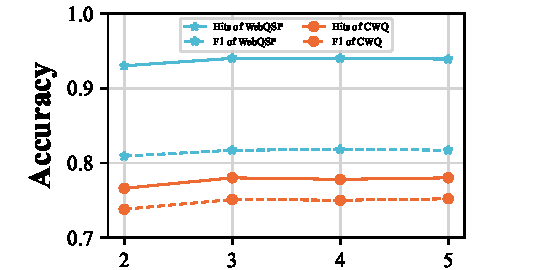
\includegraphics[width=0.265\textwidth,height=0.145\textwidth]{figure/hyper_top_k.pdf}}
%     \label{fig:mcts_top_k}
%     \hspace{-0.5cm}
%     \subfloat[Reasoning path length $L$]{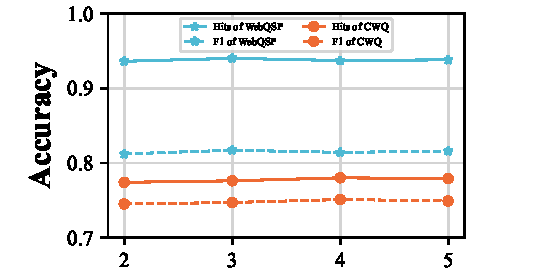
\includegraphics[width=0.265\textwidth,height=0.145\textwidth]{figure/hyper_mcts_deep.pdf}}
%     \label{fig:mcts_length}
%     \hspace{-1.3cm}

%     \caption{ Sensitivity analysis of hyperparameter on the WebQSP and CWQ datasets.}
%     \label{fig:hyper_sensitive}
%     \vspace{-0.4cm}
% \end{figure}

% \begin{table}[t]
% \centering
% \small
% \vspace{-0.1cm}
% \caption{Performance of \method{} using different LLM-based planners as backbones on the WebQSP and CWQ datasets. \textbf{Bold} values denote the best results.}
% \begin{tabular}{l|cc|cc}
% \toprule
% \multirow{2}{*}{Method} & \multicolumn{2}{c}{WebQSP} & \multicolumn{2}{c}{CWQ} \\
%  & Hits@1 & F1 & Hits@1 & F1 \\
% \midrule

% \method{} (Llama2-13B) & 91.0 & 76.7 & 73.9 & 69.5 \\

% \method{} (Qwen3-14B) & 91.5 & 77.8 & 74.4 & 70.1 \\

% \method{} (GPT 4.1-mini) & 93.1 & 80.6 & 76.1 & 72.7 \\

% \method{} (GPT 4.1) & \textbf{94.0} & \textbf{81.7} & \textbf{78.0} & \textbf{75.1} \\

% \bottomrule
% \end{tabular}
% \vspace{-0.4cm}
% \label{tab:backbone_results}
% \end{table}


\section{Conclusion}

In this work, we presented DAMR, a dynamically adaptive MCTS-based framework for knowledge graph question answering that integrates an LLM-guided planner, a context-aware path evaluator, and a dynamic pseudo-path refinement mechanism. By narrowing the search space, reducing redundant LLM calls, and continually adapting path evaluation, DAMR achieves efficient and accurate multi-hop reasoning. Extensive experiments on WebQSP and CWQ demonstrate that DAMR consistently surpasses state-of-the-art baselines in both performance and efficiency, while ablation and case studies highlight its interpretability and robustness. These results establish DAMR as a scalable solution for real-world KGQA and open avenues for extending adaptive symbolic–neural reasoning to broader domains such as scientific discovery and recommendation.

% In this work, we present \method{}, a dynamically adaptive MCTS-based reasoning framework for complex KGQA tasks. \method{} incorporates an LLM-based planner to guide top-$k$ relation expansion, a context-aware path evaluator to assess reasoning paths without further LLM queries, and a dynamic refinement module that continually adapts the evaluator using pseudo-path supervision from MCTS rollouts. This modular design enables efficient yet accurate multi-hop reasoning by narrowing the search space, reducing redundant computation, and enhancing evaluation quality. Extensive experiments on WebQSP and CWQ confirm the effectiveness and efficiency of \method{}, making it a practical and scalable solution for real-world KGQA deployment.


\bibliographystyle{plain}
\bibliography{main}
\clearpage
\onecolumn
\appendix

\section{Algorithm}\label{sec:algorithm}

\begin{algorithm}[h]
    \caption{Dynamic MCTS-based KGQA with Path Model Pretraining and Online Refinement}
    \renewcommand{\algorithmicrequire}{\textbf{Input:}}
    \renewcommand{\algorithmicensure}{\textbf{Output:}}
    \begin{algorithmic}[1]
        \REQUIRE Question $q$, knowledge graph $\mathcal{G} = (\mathcal{E}, \mathcal{R}, \mathcal{T})$, number of selected relations $k$, MCTS iterations $N$, length of reasoning path $L$
        \ENSURE Answer set $\mathcal{A}$
        
        \STATE \texttt{/ Stage 1: Path Evaluation Model Pre-training /}
        \STATE Construct reasoning path pairs $(q, p^{+}, p^{-})$ from $\mathcal{G}$ 
        \STATE Initialize path evaluation model $S(q, \cdot; \Theta)$
        \FOR{each batch in pretraining data}
            \STATE Update $S(q, \cdot; \Theta)$ by minimizing the Pair-wise Ranking loss in Eq.(4) 
        \ENDFOR

        \STATE \texttt{/ Stage 2: Dynamic MCTS Reasoning /}
        \FOR{$i = 1$ to $N$}
            \STATE \textbf{Selection:}
            Traverse the tree from root to a leaf node by selecting child nodes according to the UCT criterion in Eq.(1)
            \STATE \textbf{Expansion:}
            
            \STATE i. At the selected node, enumerate all candidate relations from current entities and use the LLM-based planner to select the top-$k$ most relevant relations
            
            \STATE ii. Expand a new child node for each selected relation
            \STATE \textbf{Simulation:}
            For each expanded node, perform a rollout by sequentially selecting relations (guided by the path evaluation model) up to $L$ hops or until a correct answer is reached
            \STATE \textbf{Backpropagation:}
            Update the value ($w_i$) and visit ($n_i$) statistics along the traversed path from the leaf node back to the root using the score from the simulation, as per Eq.(6)
            
            \STATE \textbf{Path Evaluation Model Fine-tuning:} Generate the explored pseudo-path pairs $(\hat{p}^{+}, \hat{p}^{-})$ via Eq.(5) and fine-tune  the path evaluation model $S(q, \cdot; \Theta)$ based on Pair-wise Ranking loss in Eq.(4)
        \ENDFOR

        \STATE \texttt{/ Stage 3: Answer Extraction /}
        \STATE Collect entities reached by high-scoring reasoning paths as $\mathcal{A}$
        \STATE \textbf{return} $\mathcal{A}$
    \end{algorithmic}
    \label{algo:dynamic-mcts-final}
\end{algorithm}

% \section{Complexity Analysis}

% The overall time complexity of the proposed \method{} framework is governed by its two primary online stages: the LLM-Guided MCTS Search and the interleaved Path-based Dynamic Refinement. In the MCTS Search phase, executed over $N$ iterations, the LLM-guided relation expansion incurs a total complexity of $\mathcal{O}\left(N \cdot T_{\text{LLM}}(k)\right)$, where $T_{\text{LLM}}(k)$ denotes the inference time of the LLM when provided with up to $k$ candidate relations from the Knowledge Graph (KG). The context-aware path evaluation performed during the simulation step introduces an additional cost of $\mathcal{O}\left(N \cdot k \cdot L^3 \cdot d\right)$, where $L$ is the maximum path length and $d$ is the embedding dimension. In the Path-based Dynamic Refinement stage, the evaluator is fine-tuned for $N_{\text{FT}}$ steps, with a total complexity of $\mathcal{O}\left(N_{\text{FT}} \cdot L^2 \cdot d\right)$. Consequently, the overall time complexity of \method{} is:
% $\mathcal{O}\left(N \cdot\left(T_{L L M}(k)+k \cdot L^3 \cdot d\right)+N_{F T} \cdot L^2 \cdot d\right)$.



\section{ Datasets}\label{sec:dataset}

\subsection{Dataset Description}
\begin{table}[h]
\centering
\label{tab:dataset_statistics}
\begin{tabular}{lccc}
\toprule
\textbf{Datasets} & \textbf{\#Train} & \textbf{\#Valid} & \textbf{\#Test} \\
\midrule
WebQSP     & 2,848   & 250    & 1,639  \\
\midrule
CWQ        & 27,639  & 3,519  & 3,531   \\
% \midrule
% MetaQA & 329,282 & 39,136 & 30,903 \\ 
\bottomrule
\end{tabular}
\caption{Statistics of KGQA datasets.}
\label{tab:datasets}
\end{table}


We conduct extensive experiments on two widely used multi-hop Knowledge Graph Question Answering (KGQA) benchmarks: WebQSP~\cite{talmor2018web} and CWQ~\cite{yih2016value}. The statistics of these two benchmarks can be found in Table \ref{tab:datasets}, and
their details are shown as follows:

\begin{itemize}
    \item The WebQuestionsSP (WebQSP) dataset is a widely adopted benchmark for evaluating single-hop and simple multi-hop KGQA~\cite{yih2016value}. It consists of 4,837 natural language questions annotated with corresponding SPARQL queries over the Freebase knowledge graph. The dataset is partitioned into 2,848 training, 250 validation, and 1,639 test instances.
    \item The ComplexWebQuestions (CWQ) dataset is a challenging benchmark designed for multi-hop KGQA~\cite{talmor2018web}. It comprises 34,689 questions derived from WebQuestionsSP, reformulated to include more complex and compositional queries. Each question typically requires multi-step reasoning over the Freebase knowledge graph, often involving conjunctions, comparatives, or nested logical structures. The dataset is divided into 27,639 training, 3,519 validation, and 3,531 test examples.

    % \item The MetaQA dataset serves as a large-scale benchmark for evaluating multi-hop knowledge graph question answering in the movie domain~\cite{zhang2018variational}. It comprises 399,321 automatically generated natural language questions based on the WikiMovies knowledge graph, partitioned into 329,282 training, 39,136 validation, and 30,903 test examples. The dataset is organised into three subsets according to the number of reasoning steps required to answer each question: 1-hop, 2-hop, and 3-hop. Each instance challenges models to perform compositional reasoning over complex entity and relation chains, providing a rigorous assessment of both single-step and multi-step KGQA capabilities.
\end{itemize}

\subsection{Data Processing}

Following prior work~\cite{shen2025reasoning,long2025enhancing, ma2025deliberation}, we preprocess the datasets by constructing localized subgraphs centered around each question entity to reduce the size of the search space. Specifically, for each question in WebQSP~\cite{yih2016value} and CWQ~\cite{talmor2018web}, we extract a subgraph from the Freebase knowledge graph by including all triples within a predefined number of hops from the topic entity. This approach preserves the essential context required for multi-hop reasoning while significantly improving computational efficiency. 

\section{ Baselines}\label{sec:baseline}

In this part, we introduce the details of the compared baselines as follows:

\begin{itemize}

\item \textbf{Semantic Parsing Methods.} We compare our \method{} with six semantic parsing methods:

\begin{itemize}
    \item \textbf{KV-Mem}: KV-Mem~\cite{miller2016key} introduce a neural architecture that stores facts as key-value pairs and enables question answering by attending over memory slots, directly retrieving relevant information to infer answers.
    \item \textbf{EmbedKGQA}: EmbedKGQA~\cite{saxena2020improving} enhances multi-hop question answering over knowledge graphs by leveraging pretrained knowledge base embeddings, enabling the model to reason over entity and relation representations without explicit path enumeration during answer prediction.
    \item \textbf{QGG}: QGG~\cite{lan2020query} generates query graphs to answer multi-hop complex questions over knowledge bases, formulating question answering as query graph prediction and enabling structured reasoning through graph matching and path ranking mechanisms.
    \item \textbf{NSM}: NSM~\cite{he2021improving} enhances multi-hop KBQA by leveraging intermediate supervision signals, decomposing questions into reasoning steps, and training a neural state machine to sequentially predict relations and entities for accurate path-based reasoning.
    \item \textbf{TransferNet}: TransferNet~\cite{shi2021transfernet} proposes a transparent framework for multi-hop QA over relational graphs by transferring question semantics to relation paths through interpretable path ranking and structured reasoning, enabling effective and explainable answer prediction.
    \item \textbf{KGT5}: KGT5~\cite{saxena2022sequence} formulates knowledge graph completion and question answering as unified sequence-to-sequence tasks, leveraging pre-trained language models to jointly encode input queries and generate answer entities or triples in a flexible and end-to-end manner.
    
\end{itemize}

\item \textbf{Retrieval-Based Methods.} We compare our \method{} with four retrieval-based methods:

\begin{itemize}
    \item \textbf{GraftNet}: GraftNet~\cite{sun2018open} proposes an early fusion framework that jointly encodes knowledge base facts and supporting text by constructing a heterogeneous graph, enabling effective reasoning through graph convolutional networks for open-domain question answering.
    \item \textbf{PullNet}: PullNet~\cite{sun2019pullnet} introduces an iterative retrieval mechanism that expands a query-specific subgraph by pulling relevant facts from both knowledge bases and text, enabling joint reasoning over heterogeneous evidence for open-domain question answering. 
    \item \textbf{SR+NSM}: SR+NSM~\cite{zhang2022subgraph} enhances multi-hop KBQA by first retrieving a question-relevant subgraph and then performing symbolic reasoning over it using Neural Symbolic Machines, improving efficiency and accuracy through constrained and focused logical inference.
    \item \textbf{SR+NSM+E2E}: SR+NSM+E2E~\cite{zhang2022subgraph} extends SR+NSM by enabling end-to-end training that jointly optimizes subgraph retrieval and reasoning. This integration enhances model coherence and allows better alignment between retrieved subgraphs and final answer prediction.
\end{itemize}


    \item  \textbf{General
Large Language Models (LLMs).} We compare our \method{} with six general
LLMs:

\begin{itemize}

    \item \textbf{Flan-T5-xl}: Flan-T5-xl~\cite{chung2024scaling} is an instruction-finetuned variant of the T5 model, trained on a diverse collection of tasks with natural language instructions. By leveraging large-scale instruction tuning, it improves zero-shot and few-shot performance across diverse NLP benchmarks.
    \item \textbf{Alpaca-7B}: Alpaca-7B~\cite{taori2023stanford} is an instruction-following language model fine-tuned from LLaMA-7B using self-instruct techniques. It demonstrates strong zero-shot and few-shot performance by aligning with human instructions across various NLP tasks.
    \item \textbf{Llama3-8B}: Llama3-8B~\cite{dubey2024llama} is part of the LLaMA 3 family of models, designed for improved instruction following, reasoning, and code generation. Pretrained on a high-quality corpus and fine-tuned with supervised signals, it achieves strong performance across diverse benchmarks.
    \item \textbf{Qwen2.5-7B}: Qwen2.5-7B~\cite{team2024qwen2} is a 7B-parameter instruction-tuned language model developed by Alibaba, optimized for tasks such as reasoning, code generation, and dialogue. It supports multi-turn conversation and demonstrates competitive performance on standard benchmarks.
    \item \textbf{ChatGPT}: ChatGPT~\cite{schulman2022chatgpt} is a conversational AI developed by OpenAI, based on the GPT architecture. It is designed to understand natural language, engage in dialogue, answer questions, and assist with a wide range of tasks across domains.
    \item \textbf{ChatGPT+CoT}: ChatGPT with Chain-of-Thought (CoT)~\cite{wei2022chain} prompting enhances the model's reasoning capabilities by encouraging it to generate intermediate reasoning steps before arriving at a final answer, improving performance on complex, multi-step problems.
\end{itemize}


    \item \textbf{LLMs with KG.} We compare our \method{} with fourteen LLMs with KG methods:

\begin{itemize}
    \item  \textbf{UniKGQA}: UniKGQA~\cite{jiang2022unikgqa} is a unified framework that integrates retrieval and reasoning for multi-hop question answering over knowledge graphs, combining subgraph retrieval, query decomposition, and neural reasoning in an end-to-end manner.
    \item \textbf{DECAF}: DECAF~\cite{yu2022decaf} is a joint framework for question answering over knowledge bases that simultaneously decodes logical forms and answers. By leveraging dual supervision, it enhances both symbolic reasoning accuracy and direct answer prediction in a unified architecture.
    \item \textbf{KD-CoT}: KD-CoT~\cite{wang2023knowledge} is a framework that enhances the faithfulness of large language models by guiding Chain-of-Thought reasoning with external knowledge, improving accuracy in knowledge-intensive question answering tasks.
    \item \textbf{Nutrea}: Nutrea~\cite{choi2023nutrea} proposes a neural tree search framework for context-guided multi-hop KGQA. It incrementally constructs reasoning trees by integrating question semantics and graph context, enabling efficient exploration of multi-hop paths for accurate answer prediction.
    \item \textbf{ToG}: ToG~\cite{sun2023think} is a framework that enables large language models to perform deep and responsible reasoning over knowledge graphs by combining structured graph information with iterative thinking and verification mechanisms for reliable multi-hop QA.
    \item \textbf{RoG}: RoG~\cite{luo2023reasoning} is a framework that enhances the faithfulness and interpretability of large language model reasoning by grounding multi-hop question answering on knowledge graphs, integrating symbolic path tracking with natural language generation.
    \item \textbf{KAPING}: KAPING~\cite{baek2023knowledge} introduces knowledge-augmented prompting by integrating structured triples into Chain-of-Thought (CoT) reasoning. It guides large language models to generate intermediate reasoning steps, enabling zero-shot multi-hop KGQA without task-specific fine-tuning.
    \item \textbf{ReasoningLM}: ReasoningLM~\cite{jiang2023reasoninglm} enhances pre-trained language models for KGQA by injecting subgraph structures into the input representation. It enables structural reasoning over retrieved subgraphs through a reasoning-aware encoder, improving performance on complex multi-hop queries.
    \item \textbf{FiDeLis}: FiDeLis~\cite{sui2024fidelis} proposes a faithfulness-aware KGQA framework that enhances reasoning consistency in LLMs by aligning generated logical forms with answer predictions. It introduces fidelity constraints to reduce hallucinations and improve answer correctness.
    
    % \item \textbf{PoG}: PoG~\cite{chen2024plan} is a self-correcting framework that enables large language models to perform adaptive planning over knowledge graphs by dynamically revising reasoning steps, enhancing robustness and accuracy in multi-hop question answering.
    
    % \item \textbf{RoG}: G-Retriever~\cite{he2024g} is a retrieval-augmented generation framework designed for textual graph understanding and question answering, which integrates graph-structured retrieval with language modeling to enhance context relevance and reasoning accuracy.
    %\item \textbf{EtD}: EtD~\cite{liu2024explore} is a GNN-LLM synergy framework for knowledge graph reasoning, where a GNN explores plausible reasoning paths and an LLM determines the final answer, combining structured exploration with semantic understanding.
    % \item \textbf{GNN-RAG}: GNN-RAG~\cite{mavromatis2024gnn} is a framework that integrates Graph Neural Networks with retrieval-augmented generation, enabling large language models to reason more effectively by retrieving and encoding structured knowledge from graphs for informed answer generation.
    \item \textbf{GNN-RAG}: GNN-RAG~\cite{mavromatis2024gnn} integrates graph neural networks with retrieval-augmented generation by encoding knowledge subgraphs into LLMs' context. It enables structural reasoning over retrieved subgraphs, improving answer accuracy in KGQA through explicit graph-aware representations.
    %\item \textbf{Interactive-KBQA}: Interactive-KBQA~\cite{xiong2024interactive}  is a framework that enables multi-turn interactions between large language models and knowledge bases, allowing iterative question refinement and retrieval to improve accuracy and coherence in complex knowledge-based question answering.
    \item \textbf{DoG}: DoG~\cite{ma2025debate} is a flexible and reliable reasoning framework that enables large language models to generate and evaluate multiple reasoning paths over knowledge graphs through a debate-style process, enhancing robustness and answer faithfulness.
    %\item \textbf{SubgraphRAG}: SubgraphRAG~\cite{ma2025knowledge} is a framework that leverages knowledge graph retrieval to provide structured context for large language models, enhancing their ability to align and match heterogeneous schemas accurately and interpretably.
    \item \textbf{DuarL}: DuarL~\cite{liu2025dual} is a collaborative framework that integrates GNNs and LLMs for KGQA, where GNNs capture structural semantics and LLMs perform adaptive reasoning, enabling accurate and interpretable multi-hop QA.
    \item \textbf{DP}: DP~\cite{ma2025deliberation} is a trustworthy reasoning framework that guides large language models using prior knowledge from knowledge graphs. It iteratively verifies and refines reasoning paths to enhance faithfulness, robustness, and answer accuracy in KGQA.
    %\item \textbf{RAPL}: RAPL~\cite{yao2025learning} is a framework designed for KGQA, which learns a lightweight and transferable graph retriever to efficiently select task-relevant subgraphs, enhancing both scalability and generalization across diverse questions.
    \item \textbf{RwT}: RwT~\cite{shen2025reasoning} is a faithful KGQA framework that models multi-hop reasoning as tree-structured exploration over knowledge graphs, enabling large language models to generate interpretable reasoning paths and improve answer consistency and accuracy.

\end{itemize}

\end{itemize}

\section{More experimental results}\label{sec:experiments_results}

To more thoroughly illustrate the impact of hyperparameter variations on model performance, we report detailed numerical results showing how performance fluctuates under different hyperparameter settings. As presented in Table~\ref{tab:sensitive_k} and Table~\ref{tab:sensitive_length}, these results provide a comprehensive understanding of the model’s sensitivity and stability across a range of configurations.

\begin{table}[t]
\centering
\small
\begin{tabular}{lcccc}
\toprule
\multirow{2}{*}{Method} & \multicolumn{2}{c}{WebQSP} & \multicolumn{2}{c}{CWQ} \\
 & Hits@1 & F1 & Hits@1 & F1 \\
\midrule
$k=2$ & 93.0 & 80.9 & 76.6 & 73.8 \\
$k=3$ & 94.0 & 81.7 & 78.0 & 75.1 \\
$k=4$ & 94.0 & 81.8 & 77.8 & 75.0 \\
$k=5$ & 93.9 & 81.7 & 78.0 & 75.2 \\
\bottomrule
\end{tabular}
\caption{Hyperparameter sensitivity analysis of the number of selected relations $k$ on the WebQSP and CWQ datasets.}
\label{tab:sensitive_k}
\end{table}



\begin{table}[t]
\centering
\small
\begin{tabular}{lcccc}
\toprule
\multirow{2}{*}{Method} & \multicolumn{2}{c}{WebQSP} & \multicolumn{2}{c}{CWQ} \\
 & Hits@1 & F1 & Hits@1 & F1 \\
\midrule
$L=2$ & 93.6 & 81.2 & 77.4 & 74.5 \\
$L=3$ & 94.0 & 81.7 & 77.6 & 74.7 \\
$L=4$ & 93.7 & 81.4 & 78.0 & 75.1 \\
$L=5$ & 93.8 & 81.6 & 77.9 & 74.9 \\
\bottomrule
\end{tabular}
\caption{Hyperparameter sensitivity analysis of the reasoning path length $L$ on the WebQSP and CWQ datasets.}
\label{tab:sensitive_length}
\end{table}



% \begin{table*}[t]
% \renewcommand{\arraystretch}{1.3}
% \small
% \centering
% % \vspace{-0.1cm}
% \begin{tabular}{>{\centering\arraybackslash}m{2.5cm}|p{7.6cm}}
% \toprule
% \textbf{Question} & Where does greek language come from? \\
% \hline
% \textbf{Answer} & \textcolor{red}{Attic Group} \\
% \hline
% \multirow{5}{*}{\textbf{Llama-2-13B}} & The Greek language originates from \textcolor{blue}{the Proto-Indo-European language family}, which spread to Greece around 2000 BCE. It evolved into the ancient Greek language, influenced by Mycenaean and Aeolic dialects, and eventually developed into Modern Greek. \\
% \hline
% \multirow{5}{*}{\textbf{Qwen-3-14B}} & The Greek language originates from \textcolor{blue}{the Proto-Hellenic branch of the Indo-European language family}. It evolved from the Mycenaean Greek of the second millennium BCE and became the foundation for Classical Greek, spoken in ancient Greece. \\
% \hline
% \multirow{5}{*}{\textbf{GPT 4.1}} & The Greek language originates from \textcolor{blue}{the Indo-European language family}. It developed in the southern Balkans around the 3rd millennium BCE and is the oldest recorded living language, with written records dating back to the 15th century BCE (Linear B script). \\
% \hline
% \multirow{5}{*}{\textbf{GPT 4.1-mini}} & The Greek language originates from \textcolor{blue}{the Hellenic branch of the Indo-European language family}. It developed in the region of Greece and the Aegean around the 3rd millennium BCE, evolving through ancient, medieval, and modern stages. \\
% \hline
% \multirow{2}{*}{\textbf{\method{}}} & \texttt{Path 1}: Entity (id: 120026) $\rightarrow$ base.rosetta.languoid.parent $\rightarrow$ \textcolor{red}{Attic Group}. \\
% \bottomrule
% \end{tabular}
% \caption{Case study of \method{}. We highlight the correct answers in \textcolor{red}{Red} and the wrong answers in \textcolor{blue}{Blue}.}
% \label{tab:case_study_method_2}
% \end{table*}


% \subsection{More case study}\label{sec:case_study}

% Table~\ref{tab:case_study_method_2} presents a case study comparing the answer accuracy of \method{} with general LLMs: Llama-2-13B, Qwen-3-14B, GPT 4.1-mini, and GPT 4.1. When asked about the origin of the Greek language, all baseline models generate fluent and seemingly plausible responses grounded in general linguistic knowledge, such as “Proto-Indo-European” or “Proto-Hellenic”, but fail to identify the correct answer: Attic Group. In contrast, \method{} accurately predicts the correct entity by explicitly traversing the relation path \textit{base.rosetta.languoid.parent} within the knowledge graph. This example illustrates a key advantage of \method{}: rather than relying solely on learned linguistic patterns, it performs structured reasoning over the knowledge graph, enabling precise and faithful answers to ontology-specific queries that often elude general-purpose LLMs.



\section{Prompt Template}

We provide the prompt templates used by the LLM-based planner to select the top-$k$ most relevant relations from the candidate set at each step of path expansion in Fig. 3, as part of the LLM Guided Path Expansion module.

\begin{tcolorbox}[title=Prompt Template for LLM-Guided Path Expansion, colback=white, colframe=black!75, boxrule=0.5pt, arc=2mm]

\textbf{Role} \\
You are an expert assistant for Knowledge Graph Question Answering (KGQA). Your core capability is to deeply understand natural language questions and the semantics of knowledge graph relations to find the most relevant reasoning paths.

\textbf{Task} \\
Your task is to act as a \textbf{“Relation Retriever.”} Given a natural language question and a list of candidate relations, you must analyze the semantics of the question and each relation to select up to \texttt{k} relations that are most likely to lead to the correct answer.


\textbf{Rules and Constraints}
\begin{itemize}[leftmargin=1.5em, itemsep=0pt, topsep=0pt]
    \item \textbf{Fidelity to Candidates}: Your selection of relations \textbf{MUST} come strictly from the provided \texttt{Candidate Relations} list. Do not invent or modify relations.
    \item \textbf{Quantity Limit}: Return no more than \texttt{k} relations. If multiple relations are highly relevant, order them from most to least relevant. If there are fewer than \texttt{k} relevant relations, return only those.
    \item \textbf{Output Format}: Your response \textbf{MUST} be a list of strings, containing the names of the relations you have selected.
\end{itemize}

\textbf{Example}
\begin{itemize}[leftmargin=1.5em, itemsep=0pt, topsep=2pt]
    \item \textbf{Input:}
    \begin{itemize}
        \item \texttt{Question}: "who was the president after jfk died"
        \item \texttt{Candidate Relations}: \{"government.president", "government.president.successor", "location.location.containedby", "people.person.place\_of\_birth"\}
        \item \texttt{K}: 2
    \end{itemize}
    
    \item \textbf{Output:}
\begin{verbatim}
["government.president", "government.president.successor"]
\end{verbatim}
\end{itemize}

\textbf{Your Task}
\begin{itemize}[leftmargin=1.5em, itemsep=0pt, topsep=2pt]
    \item \texttt{Question}: \{question\}
    \item \texttt{Candidate Relations}: \{relations\_list\}
    \item \texttt{K}: \{k\}
\end{itemize}

\textbf{Output:}
\begin{verbatim}
[]
\end{verbatim}
\end{tcolorbox}
\captionof{figure}{Prompt template used in the LLM-based planner to select top-k relations during reasoning.}
\label{fig:prompt_llm_planner}


\section{The Use of Large Language Models (LLMs)}

Large language models (LLMs) were only used to improve the clarity, grammar, and fluency of the manuscript. They were not involved in the development of research ideas, experimental design, data analysis, or any other aspect of the scientific content.
\end{document}
